%; whizzy chapter -dvi
% -initex iniptex -latex platex -format platex -bibtex jbibtex -fmt fmt
% 以上 whizzytex を使用する場合の設定。

%     Tokyo Debian Meeting resources
%     Copyright (C) 2012 Junichi Uekawa
%     Copyright (C) 2011, 2015, 2020 Nobuhiro Iwamatsu

%     This program is free software; you can redistribute it and/or modify
%     it under the terms of the GNU General Public License as published by
%     the Free Software Foundation; either version 2 of the License, or
%     (at your option) any later version.

%     This program is distributed in the hope that it will be useful,
%     but WITHOUT ANY WARRANTY; without even the implied warranty of
%     MERCHANTABILITY or FITNESS FOR A PARTICULAR PURPOSE.  See the
%     GNU General Public License for more details.

%     You should have received a copy of the GNU General Public License
%     along with this program; if not, write to the Free Software
%     Foundation, Inc., 51 Franklin St, Fifth Floor, Boston, MA  02110-1301 USA

%  preview (shell-command (concat "evince " (replace-regexp-in-string "tex$" "pdf"(buffer-file-name)) "&"))

%%ここからヘッダ開始。

\documentclass[mingoth,a4paper]{jsarticle}
\usepackage{monthlyreport}
% 日付を定義する、毎月変わります。
\newcommand{\debmtgyear}{2020}
\newcommand{\debmtgmonth}{11}
\newcommand{\debmtgdate}{21}
% started from zero:
% (let ((year 2020) (month 10)) (+ (* (- year 2005) 12) month -1))
\newcommand{\debmtgnumber}{191}

% Needed to import pandoc-generated LaTeX documents.
% See https://stackoverflow.com/questions/40438037/tightlist-error-using-pandoc-with-markdown
\providecommand{\tightlist}{%
  \setlength{\itemsep}{0pt}\setlength{\parskip}{0pt}}

% tikz picture の為のマクロ設定
\usepackage[dvipdfmx]{graphicx}
\usepackage{tikz}

\begin{document}

\begin{titlepage}
\thispagestyle{empty}
% タイトルページ:編集必要な部分は最初のマクロに飛ばすこと

\vspace*{-2cm}
第\debmtgnumber{}回 東京エリア Debian 勉強会資料\\
\hspace*{-2cm}

\includegraphics{image2012-natsu/dotdeb.pdf}\\
\hfill{}\debmtgyear{}年\debmtgmonth{}月\debmtgdate{}日

% ここはアップデートすること
% 全角文字にしないとフォントのサイズが合わないので注意
\rotatebox{10}{\fontsize{30}{30} {\gt Python、原稿システム特集}}\\

\vspace*{-2cm}
\hfill{}
\includegraphics[height=6cm]{image200502/openlogo-nd.eps}
\end{titlepage}

\newpage

\begin{minipage}[b]{0.2\hsize}
 \definecolor{titleback}{gray}{0.9}
 \colorbox{titleback}{\rotatebox{90}{\fontsize{80}{80} {\gt デビアン勉強会} }}
\end{minipage}
\begin{minipage}[b]{0.8\hsize}
\hrule
\vspace{2mm}
\hrule
\begin{multicols}{2}
\tableofcontents
\end{multicols}
\vspace{2mm}
\hrule
\end{minipage}

\dancersection{最近のDebian関連のミーティング報告}{杉本 典充}

\subsection{2020年10月度 東京エリア・関西合同Debian勉強会}

2020年10月17日(土)に東京エリアDebian勉強会と関西Debian勉強会の合同でオンラインによるDebian勉強会を開催しました。参加者は13名でした。

セミナーは上川さんによる「DebianでのRust」の発表を行いました。発表では Rust を始める人が読むとよいドキュメント\footnote{\url{https://doc.rust-jp.rs/}}の紹介があり、Debian で提供する Rust関連 のパッケージのインストール方法とよく利用するコマンド "cargo" の説明、発表の場でコーディングを行ってみることで参加者に Rust がどのようなプログラム言語であるかを伝えました。

その後、RustやDebianの最近の動向について情報交換を行いました。

\dancersection{事前課題}{杉本 典充}

今回の事前課題は以下です。

\begin{enumerate}
\item \url{https://mentors.debian.net/} のwebサイトを知っていますか
\item debexpo というwebアプリケーションを知っていますか
\item 次のプログラム言語でどのようにdebianパッケージが作られているか興味があるものを教えてください。
\end{enumerate}

%この課題に対して提出いただいた内容は以下です。

\begin{multicols}{2}
{\small
\begin{prework}{ ����(yy\_y\_ja\_jp) }
���ޤ���������ǤϤʤ��Ǥ���... �긵�Υ�åץȥåפǤ� /boot �ˤ� ext2
 ����¾�ˤ� ext3���Ƕ�ȤäƤ���ǥ����ȥåפǤ� /boot �ˤ� ext3 ����¾
 �ˤ� LVM ��� ext4 ��ȤäƤ��ޤ���
\end{prework}

\begin{prework}{ �����ϥ� }
�ǥե���Ȥ�ext3����
�����ǥե���ȤΤޤޡ�
(NTFS���VM���᡼�����ext3�⤢�뤱��)
\end{prework}

\begin{prework}{ yos.takahashi }
ext3/4���˻ȤäƤޤ���ext3�Υǡ�������١����ˤĤ�������Linux2011ǯ1���˼�ɮ���ޤ�����
\end{prework}

\begin{prework}{ MATOHARA }
����inode �ϳ���������Ƥ���inode ��ưŪ�˳�����Ƥ���XFS �����򤹤뤳
 �Ȥ�¿���Ǥ���NILFS �Ͼ�����Ƥߤ��ΤǤ�����mount ���˰ʲ��Τ褦�ʥ��
 ���������ФƤޤ��ݤ��ʤȻפ��ޤ�����
\begin{commandline}
$ sudo mount /dev/sdb1 /mnt
mount.nilfs2: WARNING! - The NILFS on-disk format may change at any time.
mount.nilfs2: WARNING! - Do not place critical data on a NILFS filesystem. 
\end{commandline}
����¾NotePC �Ǥ�dm-crypt �ξ�˥ե����륷���ƥ���֤��ưŹ沽�����ꡢ
 eCryptfs �ǰŹ沽�����ꤷ�Ƥ��ޤ����񤭹��߻���CPU �򤫤ʤ���񤷤ޤ��ġ�
\end{prework}

\begin{prework}{ ��ޤ� }
��ext2-$>$reiserfs-$>$jfs-$>$xfs-$>$reiserfs-$>$ext3�ȻȤäƤ��ޤ�����

����:
\begin{itemize}
 \item reiserfs: ���ե������¿���ե�����Υ������������ӥ��Ӥ��Ƥ��ɤ���
       �����������դȤ����ⵤ�������θ�μ�žȬ�ݥ����ɤˡ�����
 \item jfs: ����v1.0��̾��ä�IBM���ꥨ�ʥ��������ˤ�xfs��ƨ��
 \item xfs: fsck==true�˴�ư����������ǯ�Ȥä���ΤΥޥ�����Ĵ����0byte
       �ե��������������Ѥ���줺ƨ����
\end{itemize}
������reiser4��Ķ���Ԥ��뤦���ˤ��줬�����ʤäơ����ext3�˸��경��htree�����ä������⤦Ŵ�Ĥʤ鲿�Ǥ⤤���Ǥ��������Ȥ����Ĥ�nilfs�ʤɤ˼��Ф��Ƥ��ޤ���ext3�������noatime���٤Ǥ����������aufs���碌�Ƽ�ʬ���Ȥ��Ȥ� *strap �Ķ��򥯥����˥󥰤��Ƥ��ޤ����¸����ƥ��Ȥ������Ǥ�����Ǥ���USB�����ư�Ǥ�ͭ�ѡ�

���LVM�ǤϤʤ�MD��Ȥäƾ�Ĺ���ܥХå����åפ򤷤Ƥ��ޤ���
 MD(sda,sdb,sdc)�ǹ��ۤ����̾��MD(����)�Dz�ư���Хå����åפλ���
 attach/detach�򤹤롣�֥��å���٥�ʤΤǥꥫ�Х��FSǤ���Ǥ��������̤�
 �������¾����ˡ���ʤ�������
\end{prework}

\begin{prework}{ henrich }
�ȤäƤ���֤�NTFS��Ĺ���󤸤�ʤ��Ǥ����͡����졣
�����Ρ����Ѥο������ǥ�������ext4�ǥե����ޥåȤ��ޤ����������㤤��Ƚ��ʤ��Ȥ����������Ƥ��ޤ���
\end{prework}

\begin{prework}{ emasaka }
�Ĥ뤷��FS��ȤäƤޤ�
\end{prework}

\begin{prework}{ �ܾ� }
ext3����Ѥ��Ƥ��ޤ����ä��Ѥ�ä����ȤϤ��Ƥ��ޤ���
FS����ʤ��Ǥ������Ƕ�Lenny��2TB��HDD��Ȥä���parted�äƤλȤ��ƶä��ޤ�����
\end{prework}

\begin{prework}{ ����@������ }
���������Ū�˳��Ѥ��Ƥ���ե����륷���ƥ��ReiserFS�Ǥ���
�Ż��ǻȤäƤ�Ķ���ext3�Ǥ�����ext3���Ÿ������ǥ��㡼�ʥ뤬
����Ʋ��Ǥ������ηи��ʸŤ������ͥ�Ǥ���...�ˤ����ꡢ
���ޤ꿮�Ѥ��Ƥ��ޤ���
�����ReiserFS�Ķ��ǤϤ���ޤǤνꤤ���ʤ��Ÿ����ڤä��ꡢ
�Ƥ�HDD�����줫�����ꤷ�Ƥ��ﳲ����ä��и���̵���Τǡ�
��³Ū�˻ȤäƤ��ޤ���
��ǯ����ReiserFS�Υᥤ��ȯ��(Hans Reiser)�����ᤵ��Ƥ��ޤ������ƥʥ󥹤��ۤ��Ƥ��ޤ�����
�����������θ��ReiserFS��¾�γ�ȯ�Ԥˤ���³�����ݼ餵��Ƥ���Τǡ��¿����ޤ�����
\end{prework}

\begin{prework}{ nozzy123nozzy }
\begin{enumerate}
 \item LVM�ˤĤ��Ƥϡ�CentOS5.5��Ƴ�������Τ��Τޤޤ����Ѥ��Ƥޤ�����
       ���������ƥब��äƤ���Volume̾�ϥǥե���Ȥ�����ȡʼºݤˤ�
       kickstart�ˤơˤ��ѹ����ƻȤäƤޤ����ʾ㳲���Υ���١����˺��뤿
       ���
\item ext3�ˤĤ��Ƥϡ�debian-sid�����Τޤ޻��ꤷ�Ƥ����Τ򤽤Τޤ޻Ȥ�
      �Ƥ����ꤷ�ޤ���relatime, noatime ���餤�Ͼ����ɲä��Ƥߤ����ʡ���
      �ϻפäƤޤ���
\end{enumerate}
\end{prework}

\begin{prework}{ �ޤ��������ؤ� }
\begin{itemize}
 \item Debian�Ǥ��ä˶Ťä����Ȥ�����ext3��ȤäƤޤ������ۥޥ����qcow2
       ���᡼���ǥ��������ѻ��ʳ��ϡ�LVM�ϻȤäƤޤ���
 \item �����ǰ����ü�ʤΤϡ��������DHCP�������Ѥ�Armadillo-J�ǻȤäƤ�
       ��JFFS�Ǥ����ǥե���ȤΥե����०�����Ǥϥ�֡��Ȥ�����������
       �ƽ��������Ƥ��ޤ��Τǡ�RAM�ΰ�˽񤭤��ߡ��Ÿ��ڤäƤ�ä��ʤ�
       ���������Ǥ���Debian��udhcp�Υ������ѥå���������ӥ�ɤ��ƻȤäƤޤ���
       \footnote{\url{http://d.hatena.ne.jp/mkouhei/20080601/1212330630}}
 \item ��Debian���ߤǡ���ʬ����ǰ��֥ۥåȤʤΤ�palm webOS�Ǥ��������Ubuntu��
       �������ޥ���������Τ餷���ΤǤ�����/etc/mtab�򸫤��35�Ԥ⤢�ꡢ
       ���ʤ����֤ʹ����Ǥ��͡�
\end{itemize}
\end{prework}
}
\end{multicols}

%\dancersection{Debian Trivia Quiz}{username}
%
%Debianの昨今の話題についてのQuizです。
%
%今回の出題範囲は\url{debian-devel-announce@lists.debian.org} や \url{debian-news@lists.debian.org}などに投稿された内容からです。
%
%\begin{multicols}{2}
%%; whizzy-master ../debianmeetingresume201211.tex
% $B0J>e$N@_Dj$r$7$F$$$k$?$a!"$3$N%U%!%$%k$G(B M-x whizzytex $B$9$k$H!"(Bwhizzytex$B$,MxMQ$G$-$^$9!#(B
%

\santaku
{DebConf13 $B$N3+:ECO$H3+:EF|$O!)(B}
{$BF|K\!"El5~ET(B 6$B7n(B20$BF|(B}
{$B%K%+%i%0%"(B $B%^%J%0%"(B 7$B7n(B8-14$BF|(B}
{$B%9%$%9!"%t%)!<%^%k%-%e(B 8$B7n(B11-18$BF|(B}
{3}
{$B%K%+%i%0%"$O(BDebConf12$B$N3+:ECO$G$9!#(B
DebConf13$B$O%9%$%9$N%-%c%s%WCO$G3+:E$G$9!#(B
6/20$B$O3'$5$sM=Dj$r6u$1$F$*$-$^$7$g$&!#(B}

\santaku
{$B@$3&$N(BWeb$B%5!<%P$G:G$b?M5$$N$"$k(BLinux $B%G%#%9%H%j%S%e!<%7%g%s(B(W3Techs$BD4$Y(B)$B$O!)(B}
{CentOS}
{Debian}
{Ubuntu}
{B}
{\url{http://w3techs.com/technologies/history_details/os-linux}$B$K7k2L$N%0%i%U$,$"$j$^$9!#(B
$B8=:_(B Linux $B$r;HMQ$7$F$$$k(B web $B%5!<%P$N(B 32.9\% $B$,(B Debian $B$rMxMQ$7$F$*$j!"$=$N3d9g$O8=:_$bA}2C$rB3$1$F$$$k$=$&$G$9!#(B}

\santaku
{Debian $B%+!<%M%k%A!<%`$N%a%s%P!<$G$"$j!"(Bkernel.org $B$N(B 3.2.y $B0BDjHG7ONs$N%a%s%F%J$G$b$"$k(B Ben Hutchings $B$5$s$,<!4|(B Debian $B0BDjHG$H0l=o$K=P2Y$5$l$k(B Linux $B%+!<%M%k$K(B (3.2 $B7ONs$N(B mainline $B$K$OL5$$(B) $BDI2C5!G=$,Ek:\$5$l$kM=Dj$G$"$k$H=R$Y$F$$$^$9!#(B
$BB?$/$NDI2CE@$NCf$K4^$^$l$J$$$b$N$O2?!)(B}
{PREEMPT\_RT}
{Hyper-V guest drivers$B$N6/2=(B}
{ARM64/AArch64$B%"!<%-%F%/%A%c%5%]!<%H(B}
{C}
{Hyper-V guest drivers$B$O(Bmainline kernel$B$G(B3.2$B$K$b4^$^$l$F$$$^$9$,!"$h$j2~A1$5$l$?(B3.4$B$+$i$N=$@5$,F3F~$5$l$^$9!#(B
PREEMPT\_RT$B$O%O!<%I%j%"%k%?%$%`$r<B8=$9$k$?$a$N(BPatch$B!"(B
linux-image-rt-amd64 , linux-image-rt-686-pae $B$N(Bmetapackage$B$G;HMQ$G$-$^$9!#(B
$B?7$7$$(BARM 64$B%S%C%H%"!<%-%F%/%A%c%5%]!<%H$O(Bmainline kernel 3.7$B$+$i(B}

\santaku
{Wookey$B$5$s$,%"%J%&%s%9$7$?(Balpha$BHG$N(BDebian port arm64 image$B$O!)(B}
{Debian/Ubuntu port image}
{Debian/KFreeBSD port image}
{Debian/GnuHurd port image}
{A}
{self-bootstrapp(non x86)$BBP1~$H$N$3$H$G$9!#(B\url{http://wiki.debian.org/Arm64Port}$B$G%9%F!<%?%9$,3NG'$G$-$^$9!#(B}

\santaku
{700,000$BHVL\$N%P%0$,Js9p$5$l$?F|$rEv$F$k(B700000thBugContest$B$N7k2L$,=P$^$7$?!#$=$NM=A[F|$HJs9pF|$O!)(B}
{2012/12/12$B$rM=A[$7$?(BDavidPrevot}
{$BM=A[F|(B:2013/02/04$B!"Js9pF|(B:2013/02/14}
{$BM=A[F|(B:2013/02/07$B!"Js9pF|(B:2013/02/14}
{$BM=A[F|(B:2013/02/14$B!"Js9pF|(B:2013/02/07}
{C}
{$B:G$b6a$$(B2013/02/14$B$rM=A[$7$?(BChristian Perrier$B$5$s$,Ev$F$^$7$?!#7k2L$O(B\url{http://wiki.debian.org/700000thBugContest}$B$G8x3+$5$l$F$$$^$9!#(B
$B$^$?!"(B800,000/1,000,000$BHVL\$N%P%0$,Js9p$5$l$kF|$rEv$F$k%3%s%F%9%H(B\url{http://wiki.debian.org/800000thBugContest}$B$b3+:E$5$l$F$$$^$9!#(B}

\santaku
{master.debian.org$B$,?7$7$$5!3#$K0\9T$5$l$^$7$?!#$3$l$O2?$N%5!<%P$G$7$g$&$+(B $B!)(B}
{@debian.org$B$N%a!<%k%5!<%P(B}
{$B%Q%C%1!<%8$N%^%9%?!<%5!<%P(B}
{$B%Q%C%1!<%8$N%9%]%s%5!<(B(mentor)$B$rC5$9%5!<%P(B}
{A}
{$B8E$$%5!<%P$O%G%#%9%/>c32Ey$,$"$C$?$N$G!"<wL?$HH=CG$5$l!"%G!<%?$,B;<:$9$kA0$K?7$7$$%5!<%P$K0\9T$5$l$^$7$?!#(Bftp-master.debian.org$B$O(BDebian$B$N(B official package $B%j%]%8%H%j$G$9!#%Q%C%1!<%8$N%9%]%s%5!<(B(mentor)$B$rC5$9$N$O(Bmentors.debian.net$B!#(B }

\santaku
{pbuilder$B$K(Bclang support$B$,DI2C$5$l$^$7$?!#C/$,=q$$$?%Q%C%A$G$7$g$&$+!)(B}
{Sylvestre Ledru}
{Junichi Uekawa}
{Hideki Yamane}
{C}
{Debian$B$N(BClang$B%5%]!<%H$OCe!9$H?J$s$G$$$^$9!#(B}

\santaku
{DPN - 2013$BG/(B3$B7n(B4$BF|9f$K<h$j>e$2$i$l$?F|K\$N%$%Y%s%H$O(B}
{Open Source Conference 2013 Tokyo/Spring}
{Open Source Conference 2013 Hamamatu}
{Open Source Conference 2013 Tokushima}
{A}
{\url{http://henrich-on-debian.blogspot.jp/2013/02/open-source-conference-2013-tokyospring.html} $B>\:Y$O8e$[$I!#(B}


%\end{multicols}


% % (query-replace-regexp "<.*?>" "")
% % (query-replace-regexp "^[    ]\+" "")


%-------------------------------------------------------------------------------
\dancersection{DebianでのPython}{杉本典充}
%-------------------------------------------------------------------------------

\subsection{はじめに}

Debian では多くのプログラム言語の実行環境、ライブラリ及びアプリケーションのパッケージを多数提供しています。今回はPythonについてDebianではどのようにパッケージをメンテナンスしているのかを調べてみました。

\subsection{Pythonについて}

Python とは Debian などの linux 環境のみならず他の OS でも実行することが可能な
マルチプラットフォームのプログラミング言語の1つです。
2015年に機械学習のプラットフォームである tensorflow がオープンソース化され、 tensorflow には Python のライブラリが豊富なことから Python の人気が上がってきています。

Pythonのwebサイト(\url{https://www.python.org/}) では
初心者向けのチュートリアル\footnote{\url{https://www.python.org/about/gettingstarted/}}、
Pythonの言語仕様やクラス・関数の仕様書\footnote{\url{https://docs.python.org/3/}}などの多くの情報を公開しています。特に開発者向けの情報ではPEP(Python Enhancement Proposals)\footnote{\url{https://www.python.org/dev/peps/}}と呼ばれるPythonを
よりよくするための提案の募集と公開しており\footnote{DebianにもDEPという似たような仕組みがあります。\url{https://dep-team.pages.debian.net/}}、コーディング規約やライブラリの廃止勧告、互換性の説明など多岐にわたる情報を公開しています。


\subsection{DebianにおけるPython情報の取り扱いについて}

\subsubsection{基本な情報}

Debian における Python 関連の情報は以下ページにまとまっています。

\begin{itemize}
\item Python - Debian Wiki \url{https://wiki.debian.org/Python/}
\item Debian Python Policy \url{https://www.debian.org/doc/packaging-manuals/python-policy/}
\end{itemize}

Debian Project では、Python の実行環境をメンテナンスするチーム(cpython-team)とライブラリ及びアプリケーションをメンテナンスするチーム(Debian Python Team)の2つに分かれて活動しています。2つのチームの主な違いを表\ref{tb:pythonteam}に示します。

\begin{table}[htb]
  \begin{center}
  \caption{Debian ProjectにおけるPythonのチーム情報}
  \begin{tabular}{|c|c|c|} \hline
    チーム名 & cpython-team & Debian Python Team(DPT) \\ \hline
    役割 & 実行環境のメンテナンス & ライブラリとアプリケーションのメンテナンス \\ \hline
    メーリングリスト & debian-python@lists.debian.org & (同左) \\ \hline
    IRC & \#debian-python & (同左) \\ \hline
    wiki & - & \url{https://wiki.debian.org/Teams/PythonTeam} \\ \hline
    gitリポジトリ & \url{https://salsa.debian.org/cpython-team} & \url{https://salsa.debian.org/python-team} \\ \hline
  \end{tabular}
  \label{tb:pythonteam}
  \end{center}
\end{table}

「Debian Python Policy」\footnote{\url{https://www.debian.org/doc/packaging-manuals/python-policy/}} を読んでみて、パッケージの話で大事そうなところを以下に挙げてみます。

\begin{itemize}
\item python3 へ移行しましょう
\item python のインタプリタのディレクトリ配置やファイル名の規則(例:/usr/bin/python3、/usr/bin/python3.8)
\item python ライブラリのパスの規則(debian パッケージでは /usr/lib/python{3,2.7}/dist-packages/ 配下に配置する)
\item python のライブラリやアプリケーションの debian パッケージ名の命名規則(pythoh3 系用であれば python3-* の形式とすると、モジュール名にアンダースコアが入っている場合は debian パッケージ名ではハイフンに置換すること)
\item pythonプログラムについて
  \begin{itemize}
  \item シェバンには \#!/usr/bin/env interpreter\_name は使わないこと
  \item \#!/usr/bin/python3 または \#!/usr/bin/python3.y としてdebianが提供するデフォルトのバージョンを指定すること
  \end{itemize}
\item python の debian パッケージ化を支援するための debhelper の拡張として dh-python パッケージがある
\end{itemize}


\subsubsection{cpython-teamについて}

cpython-team チームの \url{https://salsa.debian.org/groups/cpython-team/-/group_members} に表示されるメンバーは Matthias Klose(@doko) さん1名のみです。

Klose さんが メンテナンスしている \url{https://tracker.debian.org/pkg/python3.9} を確認してみると、maintainer にはチームでなく Klose さんの名前が書いてあります。そのため 1 人でメンテナンスしているようです。

2020 年 11 月 時点の unstable においては python-2.7、3.8、3.9 のパッケージを提供しており、現在は python-3.9 のデバッグ作業を行っています\footnote{\url{https://bugs.debian.org/cgi-bin/pkgreport.cgi?tag=python3.9;users=debian-python@lists.debian.org}}。


\subsubsection{Debian Python Team(DPT)について}

Debian Python Team(DPT)のメンバーは \url{https://wiki.debian.org/Teams/PythonTeam} に記載があり、2020 年 11 月現在では 20 名でメンテナンスしているようです。チームでメンテナンスしているパッケージの一覧は次のURLで見ることができます。

\begin{itemize}
\item \url{https://qa.debian.org/developer.php?email=team%2Bpython%40tracker.debian.org}
\end{itemize}  


Debian Python Team(DPT)に参加するには チームのポリシードキュメントを読み、応諾した上で参加することを求めています。チームのポリシーを記載したドキュメントは以下のページにあります。

\begin{itemize}
\item \url{https://salsa.debian.org/python-team/tools/python-modules/blob/master/policy.rst}
\end{itemize}  

このページに記載しているポリシーにはおおよそ以下の内容が書かれています。

\begin{itemize}
\item チームへ参加方法
  \begin{itemize}
  \item 以下3つを書いたメールを debian-python@lists.debian.org へ送信する
    \begin{itemize}
    \item なぜ参加したいのか
    \item \url{https://salsa.debian.org} にログインするアカウント名
    \item ポリシードキュメント(policy.rst)を読み、受諾することの宣言
    \end{itemize}
  \end{itemize}
\item パッケージメンテナンスについて
  \begin{itemize}
  \item debian パッケージ内の debian/control ファイルの Maintainer フィールド及び Uploaders フィールドの意味
  \item git-buildpackage を使ったパッケージメンテナンスの説明
  \end{itemize}
\end{itemize}

また、Python のパッケージを作るにあたっては debian/control、debian/rules などのファイルの書き方の説明が以下のページ記載されています。

\begin{itemize}
\item \url{https://wiki.debian.org/Python/LibraryStyleGuide}
\item \url{https://wiki.debian.org/Python/AppStyleGuide}
\end{itemize}


\subsubsection{pypiパッケージをdebianパッケージに変換する}

プログラム言語にはそれぞれライブラリやアプリケーションをパッケージ化して配布するサイトを持っていることが多いです。そして Debian ではそれぞれのプログラム言語のライブラリを debian パッケージへ変換する debian パッケージを配布しており、以下のページに情報があります。

\begin{itemize}
\item \url{https://wiki.debian.org/AutomaticPackagingTools}
\end{itemize}
    
Python におけるライブラリやアプリケーションの配布サイトは \url{https://pypi.org/} が有名です。上記 URL で紹介している Python 向けの debian パッケージへの変換ツールは「python3-stdeb」 パッケージに入っている「py2dsc-deb」コマンドがよさそうに思いました\footnote{pypi2debパッケージは依存パッケージがとても多くperl関連のパッケージが大量にインストールされます。}。

試しに py2dsc-deb コマンドを使って pypi が配布するパッケージを debian パッケージに変換してみました。debian/compatバージョンは "9" として変換しているようです。

\begin{commandline}
$ sudo apt-get install python3-stdeb python-all dh-python
$ wget https://files.pythonhosted.org/packages/53/20/4019a739b2eefe9282d3822ef6a225250af964b117356971bd55e274193c/ws4py-0.5.1.tar.gz
$ py2dsc-deb ws4py-0.5.1.tar.gz
$ ls -l deb_dist
l合計 128
-rw-r--r-- 1 norimitu norimitu 38224 11月 19 13:58 python3-ws4py_0.5.1-1_all.deb
drwxr-xr-x 8 norimitu norimitu  4096 11月 19 13:58 ws4py-0.5.1
-rw-r--r-- 1 norimitu norimitu   916 11月 19 13:58 ws4py_0.5.1-1.debian.tar.xz
-rw-r--r-- 1 norimitu norimitu   869 11月 19 13:58 ws4py_0.5.1-1.dsc
-rw-r--r-- 1 norimitu norimitu  5480 11月 19 13:58 ws4py_0.5.1-1_amd64.buildinfo
-rw-r--r-- 1 norimitu norimitu  1024 11月 19 13:58 ws4py_0.5.1-1_amd64.changes
-rw-r--r-- 1 norimitu norimitu  5419 11月 19 13:58 ws4py_0.5.1-1_source.buildinfo
-rw-r--r-- 1 norimitu norimitu  1377 11月 19 13:58 ws4py_0.5.1-1_source.changes
-rw-r--r-- 2 norimitu norimitu 51408  2月 26  2020 ws4py_0.5.1.orig.tar.gz

$ cat deb_dist/ws4py-0.5.1/debian/compat
9
\end{commandline}

また、python のパッケージをインストールするコマンド "pip" でインストールしたときに binding ライブラリのコンパイルも一緒に行うライブラリ "mysqlclient" を試してみると、以下のコマンドで debian パッケージに変換できました。

\begin{commandline}
$ sudo apt-get install python3-stdeb python3-all-dev dh-python libmysqlclient-dev
$ wget https://files.pythonhosted.org/packages/a5/e1/e5f2b231c05dc51d9d87fa5066f90d1405345c54b14b0b11a1c859020f21/mysqlclient-2.0.1.tar.gz
$ py2dsc-deb mysqlclient-2.0.1.tar.gz
$ ls -l deb_dist
合計 264
drwxr-xr-x 11 norimitu norimitu  4096 11月 19 14:15 mysqlclient-2.0.1
-rw-r--r--  1 norimitu norimitu  1236 11月 19 14:15 mysqlclient_2.0.1-1.debian.tar.xz
-rw-r--r--  1 norimitu norimitu   927 11月 19 14:15 mysqlclient_2.0.1-1.dsc
-rw-r--r--  1 norimitu norimitu  6192 11月 19 14:15 mysqlclient_2.0.1-1_amd64.buildinfo
-rw-r--r--  1 norimitu norimitu  1394 11月 19 14:15 mysqlclient_2.0.1-1_amd64.changes
-rw-r--r--  1 norimitu norimitu  5795 11月 19 14:15 mysqlclient_2.0.1-1_source.buildinfo
-rw-r--r--  1 norimitu norimitu  1464 11月 19 14:15 mysqlclient_2.0.1-1_source.changes
-rw-r--r--  2 norimitu norimitu 87807  7月  3 03:55 mysqlclient_2.0.1.orig.tar.gz
-rw-r--r--  1 norimitu norimitu 90744 11月 19 14:15 python3-mysqlclient-dbgsym_2.0.1-1_amd64.deb
-rw-r--r--  1 norimitu norimitu 48584 11月 19 14:15 python3-mysqlclient_2.0.1-1_amd64.deb

$ cat deb_dist/mysqlclient-2.0.1/debian/compat
9
\end{commandline}


\subsection{終わりに}

debian における Python パッケージをどういうチームがどのようにパッケージを作成、メンテナンスしているか調べてみました。皆さんも Python や他のプログラム言語のライブラリやアプリケーションを debian パッケージ化し、debian ライフをお楽しみください。

\subsection{参考情報}

\begin{itemize}
\item \url{https://wiki.debian.org/Python/}
\item \url{https://www.debian.org/doc/packaging-manuals/python-policy/}
\item \url{https://salsa.debian.org/python-team/tools/python-modules/blob/master/policy.rst} 
\item \url{https://wiki.debian.org/Python/LibraryStyleGuide}
\item \url{https://wiki.debian.org/Python/AppStyleGuide}
\end{itemize}


%-------------------------------------------------------------------------------
\dancersection{Debian勉強会資料のディレクトリ構成変更}{上川純一}
%-------------------------------------------------------------------------------

\subsection{Debian勉強会資料ディレクトリ構成変更の目的}

Debian勉強会開始当初はそこまでファイル数が多くなかったのでディレクトリ構
成はシンプルで、画像などはその月のサブディレクトリにいれてTexファイルや
スタイルファイルなどはトップレベルに配置するというようにしていました。し
かし15年たった現在においては800以上のファイルが初期状態で配置され、
TeXコンパイルすると中間ファイルをふくめて10000近いファイル数が配置
されるようになってきました。月にTeXファイルは4個くらい追加されるので状
況はどんどん悪くなります。

\begin{itemize}
 \item debianmeetingresumeYYYYMM.tex -- TeXファイル
 \item debianmeetingresumeYYYYMM-kansai.tex -- 関西の勉強会のTeXファイル
 \item debianmeetingresumeYYYYMM-presentation.tex -- プレゼンテーション用のTeXファイル
 \item debianmeetingresumeYYYYMM-kansai-presentation.tex -- 関西の勉強会のTeXファイル
 \item imageYYYYMM/ -- 画像ファイルなどの配置場所
\end{itemize}

また、初めてチェックアウトした人がMakeコマンドをうつと8コアの十分速い最
近のマシンでも15分くらいコンパイルにかかります。遅めのマシンだと数時間
かかるということもあるようです。Git commit 際にビルドできるかどうかチェッ
クするためにpre-commit-hookを使うという運用にしていたのですが、状況によっ
てはGit commitに長時間待たされることになるのです。全体に影響を及ぼす
大掛かりな変更などもできませんでした。それは流石に不便すぎる
ので今回ソースを年ごとに分割してみることにしました。

\subsection{ディレクトリ構成変更の実際}


ディレクトリ構成は新しいファイ売るについては以下のように変更しました。

\begin{itemize}
 \item YYYY/Makefile -- そのサブディレクトリ用のMakefile。
 \item YYYY/debianmeetingresumeYYYYMM.tex -- TeXファイル
 \item YYYY/debianmeetingresumeYYYYMM-kansai.tex -- 関西の勉強会のTeXファイル
 \item YYYY/debianmeetingresumeYYYYMM-presentation.tex -- プレゼンテーション用のTeXファイル
 \item YYYY/debianmeetingresumeYYYYMM-kansai-presentation.tex -- 関西の勉強会のTeXファイル
 \item YYYY/imageYYYYMM/ -- 画像ファイルなどの配置場所
\end{itemize}

チェックアウトしたあとの一連の作業は以下のようになると思います。

\begin{commandline}
$ cd 2020
$ edit debianmeetingresume202011.tex
$ make
$ git commit 
$ git pull --rebase
$ git push
 \end{commandline}

今までディレクトリ構成の変更については何度か途中で諦めているので今回はで
きるだけ挫折しないようにやりやすいところからはじめています。まず2020
年からはじめました。2017年までさかのぼって変更しました。また方針とし
て、リファクタリングは後回しして必要なファイルはシンボリックリンクで持っ
てきています。2016年より以前はそれ以降の年から依存されているファイル
があるので移動するにはなんらかのリファクタリングが必要になるかと思います。
utils/mkdirlinks.sh にスクリプトをおいていますが、使いまわしている画像ファ
イルなどによって依存関係が結構ありました。

\begin{commandline}
    beamerthemeKansaiDebian.sty
    beamerthemeKyoto.sty
    beamerthemeTokyo.sty
    image200502
    image200607
    image200703
    image200707
    image200802
    image201006
    image2012-natsu
    kansaimonthlyreport.sty
    monthlypresentation.sty
    monthlyreport.sty
\end{commandline}

今後の課題としては、再利用しやすい画像やスタイルファイルなどについては再
利用専用のディレクトリなどに分割するのが良いかなと思っています。

\subsubsection{UTF-8化}

全員が全部のファイルをビルドさせられる状態だと文字コードの一括変換等はあ
まりやりたくなかったのですが、今回の変更で基本的には2020/サブディレクト
リだけをビルドし直せば良いようになったので一括でUTF-8に変更しました。

スクリプトを書いてfind + xargsで実行しました。
\verb!utils/convert_to_utf8.sh!

\begin{commandline}
$ find -name '*.tex' | xargs bash ./utils/convert_to_utf8.sh
$ find -name '*.sty' | xargs bash ./utils/convert_to_utf8.sh
\end{commandline}

\subsubsection{CIの有効化}

CIを有効にしたかったのですが大きすぎておそすぎるという問題がありました。
Githubにミラーを作ってそこからCloud Build連携で力技で8コアのCloud Build
インスタンスを利用して15分以内にビルドできています。結果一回30円くら
いだったと思います。

SalsaのCI \footnote{.gitlab-ci.yml 参照} では最近のサブディレクトリ
(2020, 2021)だけをビルドするようにしてみてます。dictossさん提供の
gitlab runner 経由で7分でビルドが終わっているようです。

\begin{figure}[h]
\begin{center}
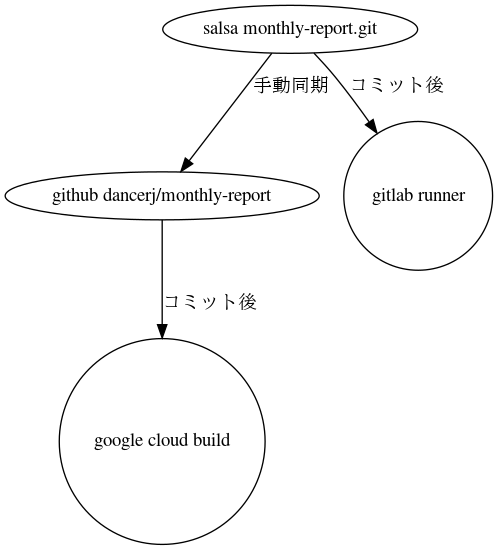
\includegraphics[keepaspectratio,width=0.5\hsize]{image202011/debci.png}
\end{center}
\caption{CIの流れ}
\label{fig:monthlyreport-ci-configuration}
\end{figure}

本当はsalsaのmasterにpushされる前にビルドのチェックを走らせたいのですが
できるのかな?

CIの設定ファイルが複数あるのも今後の課題です。

\begin{itemize}
 \item cloudbuild.yaml -- cloud buildで使っている。
 \item utils/docker/cloudbuild.yaml -- docker image 作成用
 \item .gitlab-ci.yml -- salsaの設定
 \item debian/control -- 2013年ころまで pbuilder ベースで走らせていたCI用、現在は何に利用しているのか?
\end{itemize}

最初はDebian環境にLaTeX環境のインストールとセットアップからするように設
定していたのですが、様子を見ている限りだとLaTeX関連のパッケージに何分も
か買っているようでした。Docker Imageをたまに更新するようにしてそれを利用
すればより高速になる気がしており、試しにDocker Imageを事前に作成するよう
にしたらCloud Buildの時間が13分くらいに短縮されました。

Docker Imageはとりあえず手元のraspberry pi 3 で定期的に更新するようにし
ています。

% 冊子にするために、4の倍数にする必要がある。
% そのための調整
\dancersection{メモ}{}
\mbox{}\newpage
\mbox{}\newpage
\mbox{}\newpage

\vspace*{15cm}
\hrule
\vspace{2mm}

\includegraphics[width=2cm]{image200502/openlogo-nd.eps}
\noindent \Large \bf Debian 勉強会資料\\
\noindent \normalfont \debmtgyear{}年\debmtgmonth{}月\debmtgdate{}日 \hspace{5mm}  初版第1刷発行\\
\noindent \normalfont 東京エリア Debian 勉強会 (編集・印刷・発行)\\
\hrule
\end{document}
